%%%%%%%%%%%%%%%%%%%%%%%%%%%%%%%%
%%%
%%% Research Summary
%%%
%%% Author - Steve Hurder
%%%
%%% Date Started: October 12, 2009
%%% Date Completed: November 15 , 2009
%%%%%%%%%%%%%%%%%%%%%%%%%%%%%%%% [11pt]{amsart}

\documentclass[11pt]{amsart}
% Copyright (c) 2012 Cies Breijs
%
% The MIT License
%
% Permission is hereby granted, free of charge, to any person obtaining a copy
% of this software and associated documentation files (the "Software"), to deal
% in the Software without restriction, including without limitation the rights
% to use, copy, modify, merge, publish, distribute, sublicense, and/or sell
% copies of the Software, and to permit persons to whom the Software is
% furnished to do so, subject to the following conditions:
%
% The above copyright notice and this permission notice shall be included in
% all copies or substantial portions of the Software.
%
% THE SOFTWARE IS PROVIDED "AS IS", WITHOUT WARRANTY OF ANY KIND, EXPRESS OR
% IMPLIED, INCLUDING BUT NOT LIMITED TO THE WARRANTIES OF MERCHANTABILITY,
% FITNESS FOR A PARTICULAR PURPOSE AND NONINFRINGEMENT. IN NO EVENT SHALL THE
% AUTHORS OR COPYRIGHT HOLDERS BE LIABLE FOR ANY CLAIM, DAMAGES OR OTHER
% LIABILITY, WHETHER IN AN ACTION OF CONTRACT, TORT OR OTHERWISE, ARISING FROM,
% OUT OF OR IN CONNECTION WITH THE SOFTWARE OR THE USE OR OTHER DEALINGS IN THE
% SOFTWARE.

%%% LOAD AND SETUP PACKAGES

\usepackage[margin=0.5in]{geometry} % Adjusts the margins

\usepackage{multicol} % Required for multiple columns of text

\usepackage{mdwlist} % Required to fine tune lists with a inline headings and indented content

\usepackage{relsize} % Required for the \textscale command for custom small caps text

\usepackage[pdftex]{hyperref} % Required for customizing links
\usepackage[dvipsnames]{xcolor} % Required for specifying custom colors
\definecolor{dark-blue}{rgb}{0.15,0.15,0.4} % Defines the dark blue color used for links
\hypersetup{colorlinks,linkcolor={dark-blue},citecolor={dark-blue},urlcolor={dark-blue}} % Assigns the dark blue color to all links in the template

\usepackage{tgpagella} % Use the TeX Gyre Pagella font throughout the document
\usepackage[T1]{fontenc}
\usepackage{microtype} % Slightly tweaks character and word spacings for better typography

\pagestyle{empty} % Stop page numbering

%----------------------------------------------------------------------------------------
%	DEFINE STRUCTURAL COMMANDS
%----------------------------------------------------------------------------------------

\newenvironment{indentsection} % Defines the indentsection environment which indents text in sections titles
{\begin{list}{}{\setlength{\leftmargin}{\newparindent}\setlength{\parsep}{0pt}\setlength{\parskip}{0pt}\setlength{\itemsep}{0pt}\setlength{\topsep}{0pt}}}{\end{list}}

\newcommand*\maintitle[2]{\noindent{\LARGE \textbf{#1}}\ \ \ \emph{#2}\vspace{0.3em}} % Main title (name) with date of birth or subtitle

\newcommand*\roottitle[1]{\subsection*{#1}\vspace{-0.3em}\nopagebreak[4]} % Top level sections in the template

\newcommand{\headedsection}[3]{\nopagebreak[4]\begin{indentsection}\item[]\textscale{1.1}{#1}\hfill#2#3\end{indentsection}\nopagebreak[4]} % Section title used for a new employer

\newcommand{\headedsubsection}[3]{\nopagebreak[4]\begin{indentsection}\item[]\textbf{#1}\hfill\emph{#2}#3\end{indentsection}\nopagebreak[4]} % Section title used for a new position

\newcommand{\bodytext}[1]{\nopagebreak[4]\begin{indentsection}\item[]#1\end{indentsection}\pagebreak[2]} % Body text (indented)

\newcommand{\inlineheadsection}[2]{\begin{basedescript}{\setlength{\leftmargin}{\doubleparindent}}\item[\hspace{\newparindent}\textbf{#1}]#2\end{basedescript}\vspace{-1.7em}} % Section title where body text starts immediately after the title

\newcommand*\acr[1]{\textscale{.85}{#1}} % Custom acronyms command

\newcommand*\bull{\ \ \raisebox{-0.365em}[-1em][-1em]{\textscale{4}{$\cdot$}} \ } % Custom bullet point for separating content

\newlength{\newparindent} % It seems not to work when simply using \parindent...
\addtolength{\newparindent}{\parindent}

\newlength{\doubleparindent} % A double \parindent...
\addtolength{\doubleparindent}{\parindent}

\newcommand{\breakvspace}[1]{\pagebreak[2]\vspace{#1}\pagebreak[2]} % A custom vspace command with custom before and after spacing lengths
\newcommand{\nobreakvspace}[1]{\nopagebreak[4]\vspace{#1}\nopagebreak[4]} % A custom vspace command with custom before and after spacing lengths that do not break the page

\newcommand{\spacedhrule}[2]{\breakvspace{#1}\hrule\nobreakvspace{#2}} % Defines a horizontal line with some vertical space before and after it


\newcommand{\grant}[7]{

\headedsubsection{#1}{#2--#3 (#4)} { % title, start date, end date, source
	\inlineheadsection{Investigators:}{#5}
	\vspace{1.2em}
	\inlineheadsection{Award:}{\$#6 (Share: \$#7)}
	\vspace{1.2em}
}
}

\newcommand{\colabgrant}[8]{

\headedsubsection{#1}{#2--#3 (#4)} { % title, start date, end date, source
	\inlineheadsection{Investigators:}{#5}
	\vspace{1.2em}
	\inlineheadsection{Award:}{\$#6 (Share: \$#7)}
	\vspace{1.2em}
	\inlineheadsection{Collaboration:}{#8}
	\vspace{1.2em}
}
}


\usepackage{graphicx}
\usepackage{amssymb}
\usepackage{mfirstuc}
\usepackage{colortbl}
\usepackage{epstopdf}
\usepackage{url}

\newcommand{\abr}[1]{\textsc{#1}}
\newcommand{\newcite}[2]{\capitalisewords{#1} et al.~\cite{#1-#2}}



\newcommand{\student}[1]{\vspace{.5cm}\fbox{\parbox{0.95\linewidth}{{\small
        #1}}}\vspace{.5cm}}
\providecommand{\blue}[1]{{\color{blue}{#1}}}
\providecommand{\red}[1]{{\color{red}{#1}}}
\providecommand{\green}[1]{{\color{green}{#1}}}

\begin{document}

 \title{Research Proposal: Evaluating and Enabling Human--AI Collaboration}

 \author{Jordan Boyd-Graber, University of Maryland}
%\institute{University of Colorado, Boulder CO 80309, USA}


\date{July 2022}

\maketitle

Artificial intelligence\footnote{I take a broad interpretation of
\abr{ai}; some of my examples might be better characterized machine
learning.  But rather than distracting boundary policing, I will embrace
the general term but will be specific in describing particular tools/models.}
(\abr{ai}) is ubiquitous: detecting spam e-mails, flagging fraudulent
purchases, and providing the next movie in a Netflix binge.
%
But they do not exist in a vacuum: as
Shneiderman~\cite{shneiderman-21} argues, \abr{ai} must exist
alongside humans.
%
My goal is to create metrics to measure whether \abr{ai} methods make
sense to users, helping users craft examples to advance \abr{ai}, and
applying \abr{ai} to applications that help illuminate complex social
science applications.

\section{Evaluating Interpretability}

My journey with evaluating interpretability began over ten years ago
with topic models.
%
Topic models are sold as a tool for understanding large data
collections: lawyers scouring Nordstream e-mails for a smoking gun,
journalists making sense of Wikileaks, or humanists characterizing the
oeuvre of Lope de Vega.
%
But topic models' proponents never asked what those lawyers,
journalists, or humanists needed.
%
Instead, they optimized \emph{held-out likelihood}. When my colleagues
and I developed the \emph{interpretability} measure to assess whether topic
models' users understood their outputs, interpretability and
held-out likelihood were negatively correlated~\cite{chang-09b}!
%
The topic modeling community (including me) had fetishized complexity
at the expense of usability\dots and topic modeling is not alone.

\begin{center}
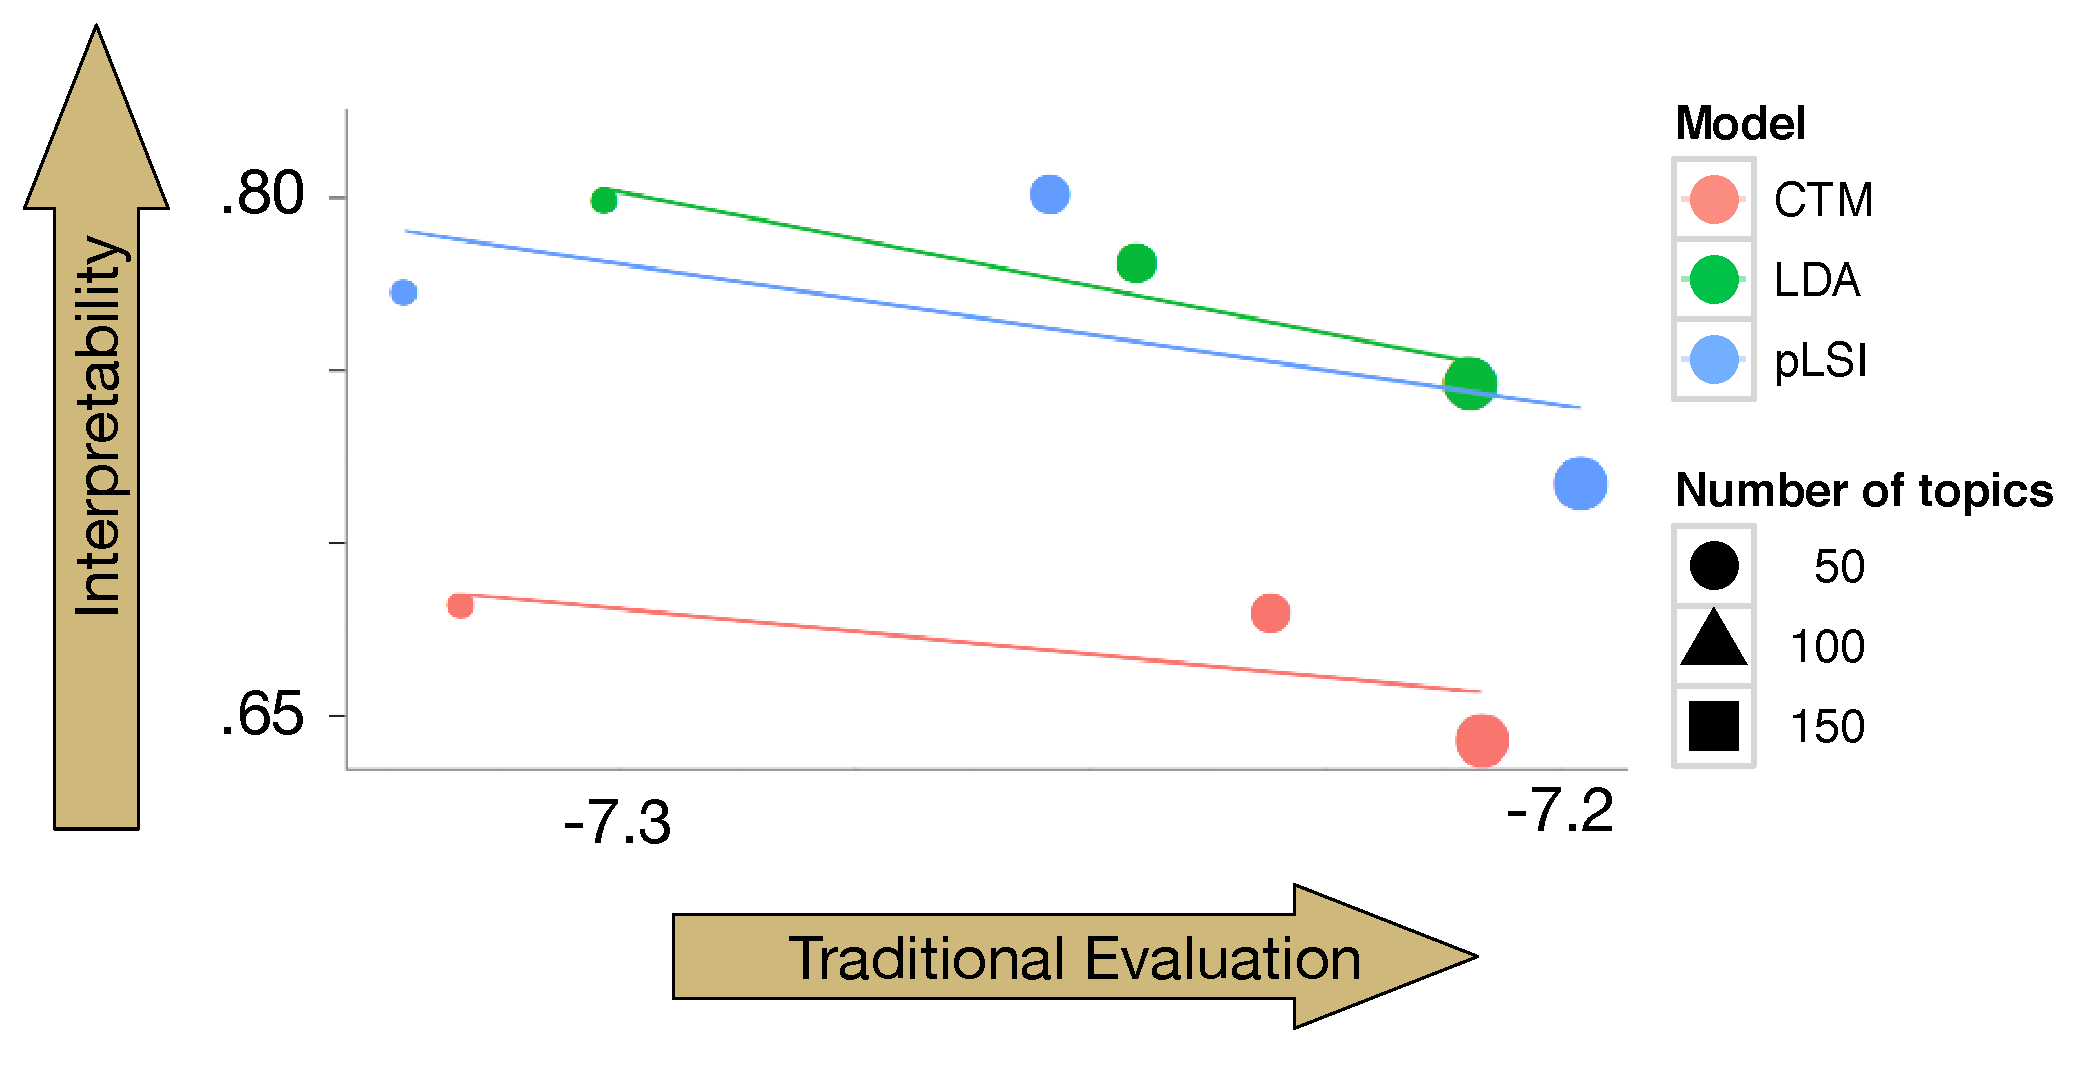
\includegraphics[width=.5\linewidth]{images/prec_ll_4}
\end{center}

Since this humbling discovery, I've built topic models that are a
collaboration between humans and computers.  The computer starts by
proposing an organization of the data.  The user separates confusing
clusters or joins similar clusters together~\cite{hu-14:itm}, and
improvement over the ``take it or leave it'' philosophy of most
machine learning algorithms.

Focusing on collaboration also requires algorithms that are low
latency (not just high throughput). We extended the
geometric interpretations of admixture models developed by Arora et
al.~\cite{arora-12} to multi-anchor topics~\cite{lund-17} and
multi-lingual topics~\cite{Yuan-18}. These are much faster than
traditional probabilistic topic models---they can handle millions of
documents in seconds---but they are less understood.  Thus, we also developed better
understanding of the projections of multilingual representations via
graph theory~\cite{Fujinuma-19} and the convergence of alternating
projections~\cite{Zhang-19}.

After we proposed our ``reading tea leaves'' evaluation, it's
heartening that \newcite{lau}{14} and their ``machine reading tea
leaves'' (which correlate with our human measures) became a standard
topic model evaluation: a survey of forty recent topic modeling
papers, {\bf all but four} use a form of their coherence evaluation.
%
However, as we argue in \newcite{hoyle}{21}, you cannot just use this
evaluation forever and forget about humans.
%
In that same survey, {\bf none} do a human evaluation.
%
As topic models evolve (e.g., incorporating
neural components), you need to validate that these automatic metrics
still correlate with whether it is useful for a human--computer
collaboration.

\section{Teaming as an Evaluation}

Within the \abr{hci} community, we have argued for the foundations of
what should go into human--computer teams: computers that incorporate
users' suggestions~\cite{kumar-19}; explanations with
accountability~\cite{smith-20}; and stable
explanations~\cite{smith-20:adherence}.

In addition to these human-centered understanding of users' needs and
desires, we've developed machine learning approaches to measure how
well users complete a task.
%
For example, for a question answering task, we measured how much the
accuracy of the human--computer \emph{team} increases with different
explanations and found that explanations help all users but that
novices are easily overwhelmed~\cite{feng-19}.
%
In follow-on work, we learned how to explicitly optimize explanations
for individual users~\cite{feng-22}.


\section{Connecting with Social Science: Pedagogy, Framing, and Deception}

The reverse of cooperation is competition; it also has much to teach computers.
%
I've increasingly looked at language-based games whose clear goals and
intrinsic fun speed research progress.
%
For example, in the board game \emph{Diplomacy}, users
chat with each other while marshaling armies for world conquest. Alliances are
fluid: friends are betrayed and enemies embraced as the game develops. However,
users' conversations let us predict when friendships break: betrayers writing
ostensibly friendly messages before a betrayal become more polite, stop talking
about the future, and change how much they write~\cite{niculae-15} in follow-on
work, we developed a dataset that predict both when users lie to each other
and when recipients of lies detect deception~\cite{Peskov-20}.
%
Diplomacy may be
a nerdy game, but it is a fruitful testbed to teach computers to understand
messy, emotional human interactions.
%
We are continuing to look into these questions with researchers from
across the nation in a new \abr{darpa} program: \abr{shade}, which
focuses on the game that were were first to highlight for its
linguistic deception as a computational task.

Recently, the use of \abr{nlp} methods in the game of Diplomacy has
been the subject of highly-publicized papers by DeepMind in Nature
Communications~\cite{kramar-22} and
Meta in Science~\cite{bakhtin-22}.
%
The Meta paper, like our 2020 paper, used a classifier to detect
deceptive statements.
%
The DeepMind paper built a game theoretic understanding of when betrayal
should happen, building on our descriptive investigation of deception
in human games.

A game with higher stakes is politics. However, just like Diplomacy, the words
that people use reveal their underlying goals; computational methods can help
expose the ``moves'' political players can use. With collaborators in political
science, we've built models that: show when politicians in debates
strategically change the topic to influence others~\cite{nguyen-12,Nguyen-14b};
frame topics to reflect political leanings~\cite{nguyen-13:shlda}; use subtle
linguistic phrasing to express their political leaning~\cite{iyyer-14a}; or
create political subgroups with larger political
movements~\cite{Nguyen:Boyd-Graber:Resnik:Miler-2015}.

Because political discourse is built on a common set of commonly
accepted facts, we have focused on developing fact checking: datasets
for general knowledge fact checking~\cite{eisenschlos-21} and climate
change fact checking~\cite{Diggelmann-20}.
%
However, because fact checking is part of an information arms race, we
need to build these examples as part of a human-in-the-loop
adversarial process, which I'm exploring in an ongoing collaboration
with journalism professor Naeemul Hassan that extends my question
answering work, which I talk about next.

\section{Human-in-the-Loop Adversarial Examples}

One of the most fun aspects of my research has been building
trivia-playing robots~\cite{boyd-graber-12,iyyer-14b,iyyer-15}; in
addition to the research, it has faced off against
former Jeopardy champions in front of hundreds high school
students.\footnote{\url{https://www.youtube.com/watch?v=LqsUaprYMOw}}
%
But after defeating some of the smartest trivia players, did I
actually believe that our system was better at question answering?
%
No!

Adversarial examples first came out of the vision community: add a
small epsilon to an example and suddenly a object detector calls a
turtle a gun~\cite{athalye-18}.\footnote{Point of personal pride: I
mentored Kevin on another previous research project~\cite{he-16}, but
I myself had nothing to do with this later adversarial work.}
%
While others have attempted to create adversarial examples for
language using paraphrasing, it's hard to know if the changes are
perceptually negligible and it's hard to ``add epsilon'' to a discrete
word.

Consistent with the theme of my research, my \abr{nsf career} grant
added a \emph{human in the loop} to generate novel adversarial language examples
that can provide new training examples to make \abr{ai} more robust
and to expose what \abr{ai} cannot (yet) do.
%
With Eric Wallace, an undergraduate student, we built a system that
could help an expert trivia question writer to stump a computer: as
the author writes the question, it shows the author what the system is
thinking~\cite{wallace-18}.
%
And it worked, even generalizing across models~\cite{wallace-19} (an
example written with an \abr{ir} model still stumps a neural model).
%
After we introduced human-in-the-loop adversarial example generation,
Meta Facebook adopted this framework with gusto~\cite{bartolo-20} in
their Dynabench framework and the Dynamic Adversarial Data Collection
workshop and call for proposals (which I'm grateful is funding our
continuing research in this area).

\section{But wait, there's more!}

Many of our best-cited papers are ``traditional'' machine learning or
natural language processing papers that do better on some task:
%
\begin{itemize*}
\item We developed the deep averaging network~\cite[\abr{dan}]{iyyer-15}, an
incredibly simple model that is still being used even in the age of
transformers~\cite{ye-22}.

\item In question answering we have proposed new evaluation
mechanisms for knowing if an answer is correct~\cite{si-21} or to
improve unsupervised retrieval of information to answer complicated
questions~\cite{elgohary-19,zhao-20,shi-20}.

\item We also introduced reinforcement learning to \emph{simultaneous
machine interpretation}~\cite{Grissom:He:Boyd-Graber:Morgan-2014}, a
  language-based task that requires significant human intuition,
  insight, and---for those who want to become
  interpreters---training.\footnote{This framework---using
  reinforcement learning to capture human strategies---was featured in
  Liang Huang's \abr{acl} keynote.} We learned tricks from
  professional human interpreters---passivizing sentences and guessing
  the verb---to translate sentences sooner~\cite{He-15}, letting
  speakers and algorithms cooperate together and enabling more natural
  cross-cultural communication.  We also use reinforcement
  learning to learn machine translation feedback from noisy
  supervision such as star ratings on a webpage~\cite{nguyen-17}.
\end{itemize*}

This work doesn't \emph{yet} fit nicely into the human--computer
collaboration narrative, but these more complex tasks are part of my
broader vision for where my research will go: state-of-the-art models
built to support human decisions, not replace them.  And that requires
the low-latency models built to react to input ``like a human''
described above.

\section{Future Work}

To advance \abr{ai}, we need to ask better questions.
%
Existing datasets are not diverse in the questions that they ask
about: Google's Natural Questions, SQuAD, and others contain entities
that are overwhelmingly male and either American on
British~\cite{gor-21}.
%
More importantly \newcite{rogers}{22} outline an ontology of what skills a computer
answering questions \emph{should} possess, and adversarial \abr{qa} generation
systems do not probe these skills.
%
Using item response theory and skilled authors, we will probe and
explicate just how capable modern \abr{ai} is and where it still needs
more work.

Where computers have strengths that go beyond what a human can do, we
will build interactive systems that help users come to a correct
answer through a process they trust.
%
This requires basic engineering---ensuring all of the components of
a system are efficient and low latency---and user modeling, as we
cannot assume that every user will have the same knowledge and
capabilities.
%
Then it will require careful vetting in diverse domains to validate
that users' skills and knowledge are actually augmented by the help of
the computer.
%
We aim to focus on multiple areas: question answering in a single
language~\cite{He-22}, question answering in a language~\cite{han-22}
or culture~\cite{peskov-21} you are unfamiliar with, and the strategic
game of Diplomacy.

As these systems become more capable and usable, we can no longer
assume that our model of the user should remain static: the user will
learn and adapt to the system.
%
This makes modeling more complicated, but it also allows for employing
these models in educational settings through examples ordered in a
curriculum: expanding the frontier of what the user knows, reinforcing
weaker knowledge, and using strategies to both educate and explain
information from the \abr{ai}.
%
This will require matching users' capabilities with what models can
offer.

But interactions with individual people are not how \abr{ai} will be a
part of 21\textsc{st} society: it will be interactions with
\emph{populations}.
%
Thus, we need to have models and systems that capture population-level
interactions.
%
Helping detect misinformation online, working collaboratively with
authors to craft effective counter-measures, and to propagate that
within a social network.
%
This builds on our fake news systems, our deception detection work,
but will also require deeper collaboration with social scientists and
journalists to develop the interfaces and the models to build
human--computer \abr{ai} that informs and helps society as a whole.


%% \vspace{12cm}

%%  \parbox{\linewidth}{I certify that this
%%   statement is a current and accurate statement of my
%%   professional record to the best of my
%%   knowledge \flushright  
\includegraphics[width=.2\linewidth]{resume_src/signature} \\
%% \flushright  (\today{})}

\clearpage

%%%%%%%%%%%%%%%%%%%%%%%%%%%%%%%%

\bibliographystyle{resume_src/splncs03}

\begin{center}
Full list of  three book chapters, eleven journal publications, and ninety-nine conference
publications at \url{http://boydgraber.org/dyn-pubs/year.html}
\end{center}

\bibliography{resume_src/journal-full,resume_src/jbg}
\noindent\rule{4cm}{0.4pt}
\end{document}
